\chapter{Einleitung}
Im Zeitalter des Internets werden immer mehr Dienstleistungen im Internet angeboten. Diese gehen weit über statische Webseiten, wie man sie aus den Anfängen des Internets kennt, hinaus. Diese sogenannten Webapplikationen sind komplexe Anwendungen, wie zum Beispiel Online Shops, soziale Netzwerke oder Onlinebanking-Portale. Aufgrund der Komplexität dieser Anwendungen, kann es schnell zu ungewollten Sicherheitslücken kommen. Dies ist kritisch, da oft sehr sensible Daten im Spiel sind. \\
Cross-Site-Scripting ist ein Angriff auf eine solche Sicherheitslücke, der in vielen modernen Webapplikationen erfolgreich durchgeführt werden kann. Dabei wird versucht auf eine fremde Website Schadcode zu hinterlegen, welcher danach von anderen Benutzern unbeabsichtigt ausgeführt wird. \\
Die Websecurity Abteilung von SAP versucht solche Schwachstellen automatisiert aufzudecken. Aus diesem Grund wurde ein modifizierter FireFox entwickelt, welcher es ermöglicht herauszufinden, welche Eingaben des Benutzers an kritischen Stellen in der Website gelangt.
\section{Aufgabenstellung}
Oft ist es sinnvoll, nicht nur eine einzige Seite auf Schwachstellen zu testen, sondern automatisiert eine Vielzahl von Seiten zu besuchen. Um dies zu ermöglichen soll im Rahmen dieser Arbeit ein Webcrawler entwickelt werden, der eine Liste von Startseiten besucht und aus diesen Verweise auf weitere Seiten extrahiert. 
Dafür muss eine Architektur gefunden werden, die sich in das aktuelle System einfügen lässt und sich gut skalieren lässt. Um diesen Webcrawler zu testen werden eine Reihe von Seiten besucht und mit den bestehenden Tools auf Cross-Site-Scripting Schwachstellen untersucht. Generell sollen aber die Möglichkeit bestehen, auch andere Testdaten während des Crawling zu sammeln und analysieren.
\section{Vorgehensweise}

\chapter{Grundlagen}
\section{Crawler}
Ein Webcrawler (oft auch Spider genannt) ist ein Computerprogramm, welches es ermöglicht, eine große Anzahl von Webseiten automatisiert zu besuchen.
\subsection{Einsatzgebiete}
Einer der bekanntesten Einsatzgebiete von Crawlern ist in Suchmaschinen. Diese bauen eine große Datenbank mit indizierten Webseiten auf und erlauben es einem Benutzer diese Datenbanken mit einer Suchanfrage zu durchsuchen. Um diese Datenbank zu füllen und aktuell zu halten wird ein Crawler verwendet, wie zum Beispiel der Googlebot der Suchmaschine Google.  [https://support.google.com/webmasters/answer/182072?hl=de] \\
Preisvergleichsportale sammeln die Preise des selben Produkts in verschiedenen Onlineshops. Somit ist es einem Kunden möglich, einfach Preise zu vergleichen, ohne die einzelnen Onlineshops zu besuchen. Das Aggregieren der Preisdaten wird oft mit Hilfe eines Webcrawlers umgesetzt. Dieser besucht alle Webseiten der Onlineshops und extrahiert für jede die gefundenen Preise. 
%[http://www.seas.upenn.edu/~cse400/CSE400_2004_2005/02writeup.pdf]%\\
Ein Crawler kann auch im Zuge eines Penetrationstest verwendet werden. Dabei wird eine Webseite bzw. Webanwendung gezielt auf Schwachstellen untersucht. Der Webcrawler hilft dabei alle Seiten der Webanwendung zu besuchen und auf Schwachstellen zu testen. Anwendungen die dies Umsetzen sind zum Beispiel \enquote{Kali Grabber} [http://tools.kali.org/web-applications/grabber], \enquote{Vega}[https://subgraph.com/vega/index.en.html] und \enquote{WebSurgery}[http://www.surgeonix.com/blog/index.php/archives/category/tools] \\
Webcrawler werden allerdings auch für kriminelle Zwecke eingesetzt. So ist es zum Beispiel möglich E-Mail-Adressen aus Webseiten zu extrahieren. Nachdem genug Seiten gecrawlt wurden, entsteht eine große Datenbank mit E-Mail-Adressen, die zum Versenden von Spam verwendet werden kann. \\
\subsection{Funktionsweise}
Die Funktionsweise eines Webcrawlers lässt sich im wesentlichen auf einen einfachen Algorithmus reduzieren. Im ersten Schritt wird eine Seite identifiziert, welche heruntergeladen werden soll. Alle Seiten, die noch besucht werden sollen, sind in einer Warteschlange gespeichert. Zu Beginn des Programms wird diese Schlange mit einer Reihe von Startseiten initialisiert, welche als Ausgangspunkt des Crawlprozesses dienen.\\
Nachdem der Schlange eine zu besuchende Seite entnommen wurde muss geprüft werden, ob das Crawlen dieser Seite überhaupt erlaubt ist. Mit der Hilfe einer robots.txt Datei oder dem HTTP Header kann festgestellt werden, ob der Webseitenbetreiber das Crawlen nicht erwünscht.
Falls die Seite besucht werden darf, wird sie komplett heruntergeladen und zu einer Liste mit besuchten Seiten hinzugefügt. Aus dem so erhaltenen HTML-Code werden nun alle Links auf der Seite extrahiert. Diese neuen Links werden der Warteschlange aus dem ersten Schritt hinzugefügt, sofern sie nicht in der Liste mit bereits besuchten Seiten enthalten sind. Somit wird verhindert, dass eine Seite mehrmals besucht wird. \\
Zum Schluss wird die heruntergeladene Seite analysiert und daraus gewonnene Informationen abgespeichert. Eine Suchmaschine könnte zum Beispiel alle Wörter die auf der Seite zu finden sind speichern. Danach beginnt der Prozess von vorne und die nächste zu besuchende Seite wird bestimmt. [http://www.ijcttjournal.org/Volume13/number-3/IJCTT-V13P128.pdf]
Bei speziellen Webcrawlern, wie zum Beispiel solche, die für Suchmaschinen eingesetzt werden, ist es außerdem nötig Seiten nach einer gewissen Zeit erneut zu besuchen, da sich der Inhalt möglicherweise geändert hat. Die Einträge in der Liste mit besuchten Seiten müssen also eine Lebensdauer zugewiesen bekommen. Läuft diese ab, so werden sie wieder in die Warteschlange des Webcrawlers eingefügt.
\subsection{Herausforderungen}
Dieser Algorithmus erscheint zunächst recht simpel, allerdings ist das World Wide Web sehr groß, wodurch sich einige Probleme ergeben. %[http://infolab.stanford.edu/~olston/publications/crawling_survey.pdf -> 1.1 Challenges] 
Um eine akzeptable Performance zu erreichen, muss der Crawlvorgang hoch parallel ablaufen. In modernen Anwendungen ist es sogar üblich diesen Vorgang auf viele verschiedene Computer zu verteilen. In einem solchen Fall spricht man dann von "Distributed web crawling". \\
Durch die enormen Datenmengen wird es auch schwierig die Datenstrukturen des Crawlers im Arbeitsspeicher zu halten. Zum Beispiel die Liste mit bereits besuchten Seiten kann sehr schnell groß werden. Diese Daten auf ein sekundäres Speichermedium zu verlagern und dabei annehmbare Performance zu behalten ist keine leichte Aufgabe. \\
Es gibt so viele Webseiten im Internet, dass selbst große Firmen wie Google mit ihren Webcrawlern diese nicht alle abdecken können. Deshalb ist es nötig gezielt Seiten zu besuchen, welche einen hohen Wert haben. Wie genau sich dieser Wert einer Seite berechnet kommt auf den speziellen Anwendungsfall des Webcrawlers an. Für Suchmaschinen sind zum Beispiel Seiten interessant, die von vielen anderen Stellen verlinkt wurden und hohe Aufrufzahlen haben. Seiten mit unwichtigem oder sogar schädlichem Inhalt müssen hingegen vermieden werden. \\
Ein hochperformanter Crawler kann schnell versehentlich einen Webserver lahm legen. Indem in kurzer Zeit zu viele Anfragen an diesen geschickt werden, kann er unter der Last zusammenbrechen. Dies kommt einem Denial of Service (DOS) Angriff gleich. Um das zu verhindern muss der Algorithmus so angepasst werden, dass nicht zu viele Anfragen an einen einzigen Webserver gestellt werden.



\section{Cross-Site Scripting}
Das "Open Web Application Security Project" (OWASP) publiziert eine Liste mit den Top 10 Sicherheitsrisiken in Webanwendungen. Sowohl in der Liste aus dem Jahr 2013, als auch im Release Candidate für das Jahr 2017, steht Cross-Site-Scripting auf dem dritten Platz. Diese Art von Sicherheitslücke ist also schon lange bekannt, aber noch immer stark verbreitet und somit relevant. \\
Beim Cross-Site Scripting, kurz XSS, versucht ein Angreifer eigenen HTML Code in eine fremde Webseite einzuschleusen. Häufig werden vom Benutzer kontrollierbare Eingaben, wie z.B. die URL, Query-Parameter, Cookies oder auch Eingabefelder, in der Webseite eingefügt. Bei der Programmierung müssen diese Eingaben auf HTML und JavaScript Code überprüft werden. Wird diese Überprüfung versäumt und die Eingabe umgeändert auf der Webseite wiedergegeben, so ist es möglich fremden Code auszuführen. \\
Das Ziel des Angreifers ist es, die Webseite so zu manipulieren, dass im Browser eines Opfers der Code des Angreifers ausgeführt wird. So kann der Angreifer das Opfer beispielsweise unbemerkt auf eine Phishing Seite weiterleiten, die zwar genauso aussieht wie die Originalseite, jedoch die Login-Daten des Benutzers abfängt. Auch denkbar ist das Stehlen der Cookies des Opfers. Dadurch kann es dem Angreifer die gelingen eine Session des Opfers zu übernehmen, ohne sich anmelden zu müssen. Es gibt noch viele weitere Angriffe, die mit Hilfe einer XSS Lücke durchgeführt werden können. Aus diesem Grund ist diese Art der Sicherheitslücke sehr problematisch.
\subsection{Cross-Site Scripting Typen}
Cross-Site Scripting Lücken lassen sich in drei Typen untergliedern: stored XSS, reflected XSS und DOM Based XSS.
\subsubsection{Stored XSS}
Bei stored XSS Angriffen wird eine Benutzereingabe an den Server gesendet, welche dort in einer Datenbank persistiert wird. Zu einem späteren Zeitpunkt besucht das Opfer eine Webseite, die diese gespeicherten Daten wieder lädt und sie ungeprüft in die Webseite einfügt. \\
Dies könnte zum Beispiel in einem Forum passieren. Der Angreifer macht einen Foreneintrag, der schädlichen JavaScript Code enthält und zum Server gesendet wird. Ruft ein anderer Benutzer diesen Forenbeitrag auf, so wird der Schadcode automatisch in die Seite eingefügt und ausgeführt. 
\subsubsection{Reflected XSS}
Wird eine Benutzereingabe unmittelbar, ohne Überprüfung, in die Webseite eingefügt, zum Beispiel als Fehlermeldung oder Suchergebnis, so spricht man von reflected XSS. Diese Benutzereingabe wird im Gegensatz zum stored XSS nirgendwo permanent gespeichert, allerdings wird sie möglicherweise trotzdem an den Server gesendet.
\subsubsection{DOM Based XSS}
Hier findet der gesamte Datenfluss von der Benutzereingabe bis zum DOM der Webseite im Browser statt. Der Schadcode des Angreifers bleibt also beim Klienten und erreicht nie den Server. Oft werden zum Beispiel Teile der URL direkt über JavaScript Funktionen wie document.write in die entsprechende Webseite eingefügt. Wird hierbei die Eingabe nicht richtig geprüft, so ist DOM Based XSS möglich.
\subsection{Beispiele}

\subsection{Taintfox}
Als Anwendungsfall des Webcrawlers dient in dieser Arbeit das automatische Finden von DOM basierten Cross-Site-Scripting Schwachstellen. Dazu wird der Taintfox verwendet, welcher diese Schwachstellen erkennen kann. \\
Der Taintfox ist eine modifizierte Version des Mozilla Firefox. Um Cross-Site-Scripting zu erkenne, werden alle Benutzereingaben markiert (tainting). Diese Eingaben kommen dabei aus unterschiedlichen Quellen, wie zum Beispiel der URL (document.location) oder den Cookies (document.cookies). Der Taintfox verfolgt den Verlauf dieser markierten Werte und merkt sich dabei, welche Funktionen auf diese angewendet werden. Landet der Wert zum Schluss in einer sicherheitskritischen Funktion wie document.write, so liegt ein potenziell kritische Datenfluss (Taintflow) vor. Die Funktion, in welcher der markierte Wert landet, nennt man auch Senke. Erkennt der Taintfox einen solchen Datenfluss, so wird das Taintfox spezifische Event taintReport ausgelöst. Auf dieses kann dann reagiert werden, um den Taintflow weiter zu analysieren.


\section{Firefox Plugins}
In diesem Abschnitt wird der generelle Aufbau von Firefox Plugins beschrieben. Für dieses Arbeit ist der Einsatz von solchen Plugins nötig, um Webseiten automatisiert im Taintfox zu öffnen. Da der Taintfox nur ein modifizierter Firefox ist, können für beide Browser die gleichen Plugins verwendet werden. In der Firefox Dokumentation ist statt Plugin auch oft die Rede von Add-On. Diese beiden Begriffe werden im weiteren Verlauf der Arbeit synonym verwendet. \\
Für die Entwickelung von Firefox Plugins gibt es zwei Optionen: das Add-On SDK und die Webextension API. Beide Ansätze werden im Folgenden kurz angesprochen.
\subsection{Firefox Add-On SDK}
Das Firefox Add-On SDK ist lange Zeit die einzige Möglichkeit gewesen, um Plugins für den Firefox zu erstellen. Es bietet eine High Level Javascript API, mit welcher es möglich ist Tabs zu öffnen, das DOM zu manipulieren, Stylesheets zu ändern und vieles mehr. Eine Low-Level-API bietet zusätzlich tiefen Zugriff auf Firefox interne Schnittstellen, um zum Beispiel alle HTTP-Abfragen abzufangen. Mit Hilfe von XPCOM, einem Komponentenmodell von Mozilla, ist es möglich vom JavaScript Code aus, auf viele interne C++ basierte Komponenten zuzugreifen. Dadurch ist es Plugins möglich den Firefox stark anzupassen. Dies ist ein Vorteil, der den Firefox lange Zeit von andern Browsern abgehoben hat. \\
Diese Starke Individualisierbarkeit hat allerdings auch Nachteile. So ist es zum Beispiel auch Schadware möglich, sensible APIs des Firefox zu verwenden. Auch das einführen von neuen Technologien in den Firefox ist schwierig, da die Abhängigkeiten zwischen den Komponenten unübersichtlich sind. Aus dieses Gründen hat sich Mozilla dazu entschieden, in zukünftigen Versionen das Addon-SDK nicht mehr vollständig zu unterstützen. [https://blog.mozilla.org/addons/2015/08/21/the-future-of-developing-firefox-add-ons/]
\subsection{WebExtension API}
Die WebExtension API ist der Nachfolger des Add-On SDKs. Auch mit ihr lassen sich Plugins erstellen, die typische Browserfunktionalitäten ansteuern. Da die WebExtension API zum größten Teil kompatibel mit der Extension API des Chrome ist, sind die damit erzeugten Plugins Browserunabhängig und laufen somit auch im Chrome, Opera und Microsoft Edge. \\
Zum Zeitpunkt, zu dem diese Arbeit geschrieben wurde, ist die WebExtension API allerdings noch nicht ganz vollständig und tiefe Eingriffe in den Firefox sind nicht mehr möglich. Trotzdem empfiehlt Mozilla den Umstieg auf WebExtensions, da dies der zukünftig unterstützte Weg ist, Plugins für den Firefox zu erstellen.
\subsection{Plugin Aufbau}
Der Aufbau eines Firefox Plugins mit Hilfe des Firefox SDK und der WebExtension API sind grundlegend gleich. Der Code ist in zwei getrennte Bereiche geteilt. Der Grundcode des Plugins hat Zugriff auf alle Firefox APIs und kann diese nutzen, um zum Beispiel neue Tabs zu öffnen, Benachrichtigungen anzuzeigen oder das Kontextmenü zu erweitern. Dieser Code kann zwar eine neue Seite aufrufen, allerdings kann nicht direkt auf den Inhalt dieser Seite zugegriffen werden. Um genauer zu sein gibt es keinen Zugriff auf das DOM der geladenen Seite. \\
An dieser Stelle kommen sogenannte "Content Scripts" zum Einsatz. Diese haben Zugriff auf den Webinhalt und verhalten sich wie ein Script, welches auf der entsprechenden Seite eingebettet ist. Der Grundcode kann diese Content Scripts in beliebe Webseiten injizieren, um so gewisse Aufgaben auf dieser Seite zu erledigen. Die Kommunikation zwischen dem Grundcode und dem Content Script findet dabei über ein port Objekt statt, welches das asynchrone Versenden von Nachrichten zwischen den beiden erlaubt. Abbildung XXX illustriert wie die Methoden emit und on des port Objekts verwendet werden, um zu kommunizieren.
%[https://developer.mozilla.org/en-US/Add-ons/SDK/Guides/Content_Scripts]

\begin{figure}
	\centering
	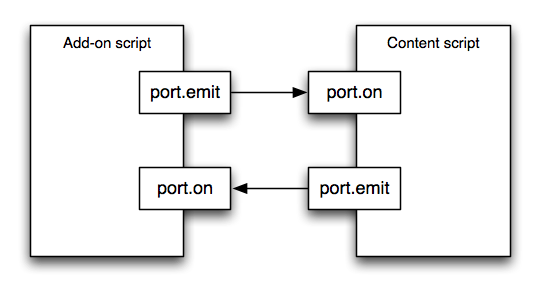
\includegraphics[width=0.8\textwidth]{Bilder/content-scripting-overview.png}
	\caption{Kommunikation mit Hilfe von Ports}
\end{figure}

\chapter{Entwurf}
\section{Anforderungsanalyse}
Im Gespräch mit der Web-Security Abteilung von SAP wurden eine Reihe von Anforderungen an den Webcrawler erarbeitet. Die folgende Liste beschreibt diese in ein paar kurzen Sätzen und gibt jeder Anforderung eine eindeutige Kennung (A + Zahl), sodass auf sie an späteren Stellen dieser Arbeit referenziert werden können. Sie sind dabei in keiner besonderen Reihenfolge gelistet, sondern alle wichtig, um den Webcrawler effektiv einsetzen zu können.
\begin{description}
	\item[ A1 ] Der Crawlvorgang soll gestartet werden können, indem eine Liste von URLs angegeben wird, die als Startseiten verwendet werden. Die Liste von URLs soll als CSV-Datei abgelegt sein. Durch eine Kommandozeilenoption kann der Pfad zu dieser Datei beim Start mit übergeben werden. Alternativ kann auch nur eine einzige URL direkt in der Kommandozeile angegeben werden
	\item[ A2 ] Nachdem der Crawler gestartet wurde, soll dieser automatisch alle Startseiten besuchen und aus diesen weitere URLs extrahieren, die danach besucht werden.
	\item[ A3 ] Das Besuchen einer Webseite soll im Taintfox erfolgen. Das heißt sie wird in einem Tab normal geöffnet, wodurch unter anderem auch alle eingebetteten JavaScript Dateien ausgeführt werden. 
	\item[ A4 ] Auf jeder Webseite, die vom Webcrawler besucht wird, soll ein Analyseplugin ausgeführt werden können, welches ebenfalls im Taintfox installiert ist. Erst wenn dieses mit der Bearbeitung der Seite fertig ist, darf sie vom Webcrawler geschlossen werden.
	\item[ A5 ] Das Analyseplugin kann dem Webcrawler zu jeder besuchten Webseite ein Datenpaket mit Analyseergebnissen übergeben. Diese Daten sollen dann zur späteren Weiterverarbeitung zentral in einer Datenbank abgelegt werden.
	\item[ A6 ] Es soll eine Option geben, die es erlaubt auf allen Seiten keine externen Links zu verfolgen. Dies ist Sinnvoll, da so die ursprünglichen Startdomains nicht verlassen werden. Somit sind die Crawlergebnisse von mehreren Crawlvorgängen auf dem gleichen Datensatz besser zu vergleichen. Auf einer fiktiven Webseite \enquote{www.webseite.co.uk} sollen also Beispielsweise folgende Links ignoriert werden: \\ \enquote{www.anders.co.uk/home}, \enquote{www.webseite.de/123}, \enquote{www.webseite.uk}. Diese Links hingegen, sollten normal weiterverfolgt werden: \\  \enquote{www.webseite.co.uk/home},  \enquote{www.subdomain.webseite.co.uk/123}. \\
	Genauso soll es auch möglich sein ausschließlich externe Links zu verfolgen. Dies kann zum Beispiel sinnvoll sein, wenn versucht wird so viele verschiedene Domains wie möglich zu erreichen.
	\item[ A7 ] Es soll eine maximale Suchtiefe angegeben werden können. Sind alle Webseiten besucht, ist der Crawlvorgang beendet. Die Startseiten besitzen die Tiefe 0. Die Webseiten, welche von den Startseiten aus erreicht wurden, haben dann entsprechend die Tiefe 1. Setzt man als maximale Tiefe 0, so werden nur alle Startseiten besucht und keine Links extrahiert. Es findet dann also kein wirkliches Crawling mehr statt, sondern ein automatisiertes Besuchen aller Seiten in einer vorgegebenen List.
	\item[ A8 ] Der Crawler soll horizontal skalierbar sein. Das heißt, es soll möglich sein mehrere Taintfox Instanzen zu starten, die alle an dem Crawlprozess teilnehmen. Dies soll auch möglich sein, wenn diese Instanzen auf unterschiedlichen Rechner laufen. Um den Crawlprozess zu beschleunigen, kann also nicht nur die Hardware eines Computers verbessert werden (vertikale Skalierung), sondern auch mehr Rechner angeschlossen werden.
	\item[ A9 ]Es soll möglich sein den Crawlprozess zu stoppen und an einem späteren Zeitpunkt fortzusetzen. Wird der Crawler gestoppt, so gibt es einige Webseiten, die schon an eine Taintfox Instanz geschickt wurden und dort gerade geladen werden, aber noch keine Ergebnisse zurück geliefert haben. Diese Seiten sollen beim Fortsetzen des Crawlvorgangs wieder als unbesucht eingestuft werden, sodass sie nochmals an eine Taintfox Instanz verteilt werden.
	\item[A10] Das Laden von sehr viele Webseiten hintereinander kann die Netzwerkverbindung oft stark belasten. Darum kann es sein, dass einige Webseiten vom Taintfox nicht erreicht werden können und es einen entsprechenden Timeout-Fehler gibt, obwohl die Webseite eigentlich online ist. Damit diese Seiten nicht durch einen Timeout übersprungen werden, soll der Webcrawler sich alle Webseiten, auf denen ein Fehler aufgetreten ist, merken. Später können diese dann erneut besucht werden.  
\end{description}


\section{Bestehende Umgebung}
In diesem Abschnitt wird nun zuerst die bestehende Umgebung beschrieben. Damit sind die einzelnen Komponenten und Tools, die bereits existieren, und deren Zusammenarbeit gemeint. Die Abbildung XXX zeigt ein Diagramm mit den einzelnen Komponenten. Wie zu sehen ist, existiert bereits ein Plugin für den Taintfox mit dem Namen "Taintnotifier". Dieses Plugin reagiert auf das taintreport Event des Taintfox. Um zu überprüfen, ob es sich bei dem gefundenen Taintflow um eine echte Schwachstelle handelt, die ausgenutzt werden kann, gibt es einen extra Validierungsservice. Das Plugin sendet diesem die potenzielle Schwachstelle per HTTP. Der Service verwendet PhantomJS, um verschiedene Angriffe auszuprobieren, ohne einen kompletten Browser nutzen zu müssen. Sobald die Validierung abgeschlossen ist, werden die Ergebnisse an das Plugin zurückgeliefert. Alle Taintflows, die auf einer Webseite gefunden wurden, werden zusammen mit den entsprechenden Validierungsergebnissen in den Entwicklertools angezeigt. \\
Das Taintnotifier Plugin bietet außerdem die Möglichkeit einen export Server anzugeben. An diesen werden per Http alle Funde gesendet, wo sie dann in einer MongoDB gespeichert werden. Später können diese Informationen dann über eine Weboberfläche abgerufen werden. \\
Dieser Aufbau erlaubt es einem Benutzer das Taintnotifier Plugin zu installieren und spezielle Seiten gezielt aufzurufen, um diese auf Schwachstellen zu testen. Wie in der Aufgabestellung bereits angesprochen, soll dieser Prozess nun automatisiert werden, damit viele Seiten in kurzer Zeit überprüft werden können.

\begin{figure}[H]
	\centering
		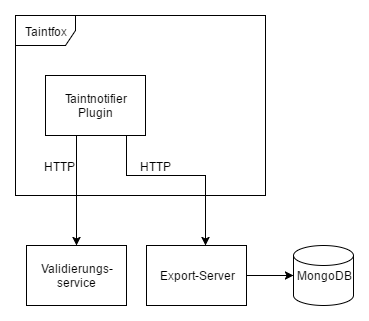
\includegraphics[width=0.8\textwidth]{Bilder/AlteUmgebung.png}
	\caption{Diagramm mit Komponenten der bestehenden Umgebung}
\end{figure}

\section{Webrawler Architekturen}
Anforderung A8 verlangt, dass der Crawlvorgang beschleunigt werden kann, indem mehrere Taintfox Instanzen gestarten werden, die alle am Crawlprozess teilnehmen. Jeder dieser Instanzen wird als Arbeiter bezeichnet. \\
Es muss gewährleistet werden, dass keine Webseite doppelt besucht wird. Die einzelnen Arbeiter müssen sich in irgendeiner Form darüber verständigen, wer für welche URLs zuständig ist. 
Es handelt sich also um "Distributed Web Crawling", da viele einzelne Prozesse verwendet werden, um das Crawlen zu beschleunigen. 
Cho and Garcia-Molina haben in diesem Umfeld 3 Typen von verteilten Crawlern erforscht: %[http://ilpubs.stanford.edu:8090/733/1/2002-9.pdf]
\begin{description}
	\item[Independent] 
	Bei diesem Typ von Crawlern sind die einzelnen Arbeiter vollkommen unabhängig voneinander und es findet keinerlei Kommunikation statt. Jeder Arbeiter erhält zu Beginn eine Liste von URLs, die er besucht, ohne sich mit anderen Arbeitern zu verständigen. Dabei kann es dazu kommen, dass es Überlappungen gibt und die gleiche Seiten von verschiedenen Arbeiter besucht wird. Dieser Ansatz ist nur sinnvoll, wenn davon ausgegangen werden kann, dass diese Überlappung nicht signifikant ist.
	\item[Dynamic assignment]
	Bei diesem Aufbau gibt es zusätzlich zu den Arbeitern einen zentralen Koordinator. Dieser hält fest welche Seiten schon besucht wurden und speichert die URLs der noch unbesuchten Seiten. Die Arbeiter erhalten dann nur noch Arbeitspakete mit einer Liste von URLs, die untersucht werden sollen. Hat ein Arbeiter dies getan, schick er alle gefundenen URLs zurück. Die Arbeiter nehmen hier also eine sehr passive Rolle ein und bearbeiten nur die Anfragen des Koordinators. Es kann zusätzlich eine dynamische Lastverteilung implementiert werden. Ist ein Arbeiter beispielsweise besonders schnell, so können ihm größere Arbeitspakete zugewiesen werden. Falls nötig, können sogar zur Laufzeit weitere Arbeiter hinzugefügt oder abgeschaltet werden\\
	Problematisch ist bei diesem Ansatz nur, dass alle Anfragen über den Koordinator gehen und dieser dadurch schnell zum Flaschenhals der Anwendung wird. Das System kann dann nicht mehr über die Anzahl der Arbeiter horizontal skaliert werden, da der Koordinator nicht schnell genug neue Arbeitspakte verteilen kann.
	\item[Static assignment] 
	Hier wird kein zentraler Koordinator benötigt, da es eine feste Regel gibt, die jede URL einem Arbeiter zuweist. Es kann zum Beispiel eine Hash-Funktion auf die URL angewendet werden, um dann jedem Arbeiter ein festen Bereich im Werteraum des Hash zuzuweisen. Dadurch ist es dann möglich festzustellen, von welchem Arbeiter eine bestimmte URL verarbeitet werden soll. Da es passieren kann, dass ein Arbeiter eine URL findet, die einem anderen Arbeiter zugewiesen ist, muss es eine Möglichkeit geben, die URLs zwischen den Arbeitern auszutauschen.
\end{description}

Im Rahmen dieses Projektes wurde sich für einen verteilten Crawler mit dynamischer Zuweisung (dynamic assignment) entschieden. Komplett unabhängige Arbeiter kommen nicht in Frage, da die Überlappung zu hoch ist. Eine statische Zuweisung ist schwer umzusetzen, da die einzelne Arbeiter dafür untereinander kommunizieren müssten. \\
Bei der dynamischen Zuweisung kann der Koordinator zwar zum Flaschenhals werden, allerdings ist dies unwahrscheinlich, da die Analyse einer Seite oft mehrere Sekunden in Anspruch nimmt. Dadurch brauchen die Arbeiter vergleichsweise lange, um ein Arbeitspaket zu bearbeiten und der Koordinator wird nicht überlastet. \\
Die Aufteilung in einen Koordinator-Server und vielen Arbeiter ist außerdem Hilfreich, um die Anforderung A5 umzusetzen. Dabei ging es darum die Analyseergebnisse von jeder Seite an einer zentralen Stelle zu speichern. Die einzelnen Arbeiter können dafür einfach die Daten an den Koordinator schicken, welcher sie dann in einer Datenbank ablegt.


\section{Neue Umgebung}
Aufgrund der Anforderungen des Webcrawlers muss die bestehende Umgebung geändert werden. Abbildung XXX zeigt ein Diagramm mit allen wichtigen Komponenten und wie diese miteinander interagieren. In den folgenden Abschnitten werden nun die einzelnen Komponenten genauer beschrieben.

\begin{figure}
	\centering
	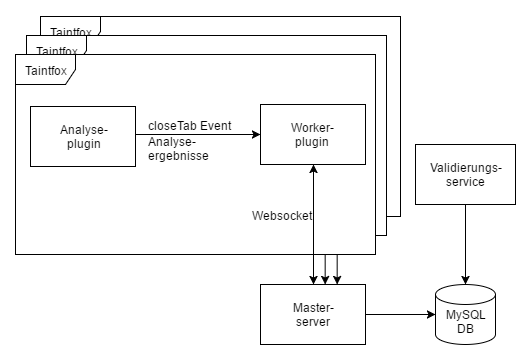
\includegraphics[width=0.9\textwidth]{Bilder/NeueUmgebung.png}
	\caption{Diagramm mit Komponenten der neuen Umgebung}
\end{figure}

\subsection{Master-Server}
In Abschnitt XXX wurde sich für ein Crawler mit dynamischer Zuweisung entschieden. Bei dieser Crawlerarchitektur gibt es einen zentralen Koordinator. Diese Rolle übernimmt in der neuen Umgebung der Master-Server. Er steuert den Crawlprozess, indem er alle bereits besuchten URLs speichert, die Warteschlange mit neuen URLs verwaltet, Arbeitspakete an die Arbeiter verteilt und die Analyseergebnisse jeder besuchten Webseite speichert. Realisiert wird der Master-Server durch eine NodeJS Anwendung. Der Master-Server ist an eine Datenbank angebunden, die verwendet wird, um Daten wie die bereits Besuchten Seiten, unbesuchte Seiten und Analyseergebnisse permanent zu speichern. Dies ist nötig, da der Webcrawler, wie in Anforderung A9 beschrieben, nach einem Neustart an der Stelle weiter machen soll, an der er aufgehört hat.
\subsection{Worker-Plugin}
Innerhalb des Taintfox kann man im Diagramm XXX eine Komponente mit dem Namen \enquote{Worker-Plugin} sehen. Dabei handelt es sich um ein Firefox Plugin, welches als Arbeiter für den Webcrawler fungiert. Es nimmt die Arbeitspakete entgegen und weist den Taintfox an, die einzelnen Seiten zu besuchen. Im Diagramm ist angedeutet, dass es mehrere Taintfox Instanzen mit entsprechenden Worker-Plugins geben kann. Jeder dieser Arbeiter meldet sich bei seinem Start bei dem Master-Server an. \\
Für die Kommunikation zwischen Arbeiter und Master kommen zwei Protokolle in Frage: HTTP und Websocket. Bei HTTP handelt es sich um ein Request/Response Protokoll. Der Klient stellt also eine Anfrage an den Server und bekommt von diesem eine Antwort. Jeder Arbeiter müsste also ein Polling durchführen, um neue Arbeitspakete zu erhalten. Das bedeutet sobald ein Arbeiter sein Arbeitspaket bearbeitet hat, muss er in gewissen Zeitabständen den Master nach einem neuen Fragen. \\
Polling ist generell keine besonders schöne Lösung. Abhilfe schafft das Websocket Protokoll. Hier ist es dem Server Möglich direkt Nachrichten an einen Klienten zu senden, ohne das dieser eine explizite Anfrage gestellt hat. Diese Art des Datenaustausches nennt man "pushing". Für dieses Projekt wurde sich für Websockets entschieden, damit eine bidirektionale Verbindung zwischen Master und Arbeiter möglich ist.\\
\subsection{Analyseplugin}
Der Master-Server und das Worker-Plugin stellen die Hauptkomponenten des Crawlers da. Diese können unabhängig betrieben werden, um eine Reihe von Seiten zu besuchen. Wie in Anforderung A4 beschrieben, soll es aber auch die Möglichkeit geben ein Analyseplugin zu verwenden, welches die besuchten Seiten auf bestimmte Schwachstellen untersucht. Die konkrete Implementierung des Analyseplugins hängt dabei vom Anwendungsfall ab. Für diese Arbeit wird ein Analyseplugin erstellt, welches die taintreport Events des Taintfox sammelt, um diese später auf Cross-Site-Scripting Schwachstellen zu prüfen.
Das Analyseplugin wird zusätzlich zum Worker-Plugin im Taintfox installiert. Sobald die Analyse abgeschlossen ist, muss dem Worker-Plugin mitgeteilt werden, dass diese Webseite nun geschlossen werden kann, sodass die nächste Seite aufgerufen wird. Anforderung A5 beschreibt die Möglichkeit, dass dabei Analyseergebnisse zu dieser Webseite mitgegeben werden. Diese werden dann vom Worker-Plugin weitergeleitet zum Master. Die Kommunikation zwischen den beiden Plugins findet dabei über ein internes Eventsystem im Taintfox statt.\\
\subsection{Validierungsservice}
In der vorherigen Umgebung wurde jedes Analyseergebnis auch gleich vom Validierungsservice überprüft, um festzustellen, ob es sich um eine tatsächliche Sicherheitslücke handelt. Da dieser Prozess aber auch unabhängig vom Crawling stattfinden kann und dies nur unnötig verlangsamt, wurde er ausgelagert. Während des Crawlprozesses werden die potentiellen Lücken, die das Anayseplugin findet, an den Master-Server weiter gereicht, welcher sie in der Datenbank speichert. Dort können sie später von dem Validierungsservice abgerufen werden, ohne den Crawlprozess zu stören. Auch der Validierungsservice ist, wie das Analyseplugin, abhängig von dem konkreten Anwendungsfall. Da in dieser Arbeit Cross-Site-Scripting Schwachstellen aufgedeckt werden sollen, wird der bestehende Validierungsservice mit dem PhantomJs Backend verwendet. Es sind allerdings auch Anwendungsfälle denkbar, bei denen keine Validierung nötig ist, aber die Analyseergebnisse stattdessen anders weiterverarbeitet werden.

\chapter{Implementierung}
Nachdem im vorhergehenden Kapitel die einzelnen Komponenten der Webcrawler Architektur erarbeitet wurde, wird in diesem Kapitel nun die Implementierung des Masterservers und Workerplugins genauer betrachtet. Diese beiden Komponenten stellen den Kern des Webcrawlers dar und sind unabhängig von dem speziellen Anwendungsfall für den der Crawler eingesetzt werden soll.
\section{Master Server}
\subsection{Klassendiagramm}
Die Klasse Crawler stellt die zentrale Klasse des Crawlers da. Sie bietet die Methode start, mit der ein neuer Crawlprozess gestartet werden kann. Dabei muss ein Array mit entsprechenden Startwebseiten angegeben werden. \\
Für jeden Arbeiter, der sich bei dem Master-Server registriert hat existiert eine Instanz der Klasse Worker. Diese kümmert sich um die Verwaltung der Websocketverbindung und speichert wie viele Arbeitspakte momentan bearbeitet werden. Dadurch kann abgefragt werden, ob dieser Arbeiter noch ein weiteres Arbeitspaket verarbeiten kann. \\
Alle Worker werden von der Klasse WorkerPool verwaltet, welche Auskunft darüber gibt, ob es momentan einen Worker gibt, der noch Arbeit benötigt und es durch die Methode processWorkPackage erlaubt ein Arbeitspaket zu verarbeiten. Dabei wird vom WorkerPool entschieden welcher Arbeiter am besten dafür geeignet ist. An dieser Stelle kann also ein Loadbalancing eingebaut werden, um die Arbeiter gleichmäßig auszulasten.

Die Klasse PageRepository hat die Aufgabe alle gefundenen Webseiten zu verwalten. Mit Hilfe der addPages Methode können neu gefundene Webseiten hinzugefügt werden. Diese sind dann zunächst als unbesucht markiert. Wird versucht eine Webseite hinzuzufügen, die bereits enthalten ist, wird diese ignoriert.\\
Die Methode makeWorkPackage erlaubt es dann ein Arbeitspaket einer beliebigen Größe zu erstellen. Dabei werden entsprechend viele Seiten, die noch als unbesucht markiert sind, zurückgeliefert. In dieser Funktion kann also definiert werden, welche Webseiten als nächstes bearbeitet werden sollen. Es gibt verschiedene Strategien, wie dies bestimmt werden kann. Diese Strategien werden in Abschnitt XXX genauer beschrieben.\\
Durch das Aufrufen der Methode setPagesVisited kann eine Liste von Webseiten als besucht markiert werden. \\
Mit welcher unterliegenden Technik die Klasse PageRepository implementiert wurde ist dabei von außen nicht zu erkennen. Für diese Projekt wurde sich für eine Implementierung mit einer MySQL Datenbank entschieden, da die gefundenen Seiten so persistent gespeichert werden und der Crawlprozess somit auch nach einem Neustart des Master-Servers fortgesetzt werden kann. Es ist aber durchaus vorstellbar zu einem späteren Zeitpunkt noch andere Implementierungen bereit zu stellen. So zum Beispiel eine In-Memory-Datenbank, wodurch die Abfragen an das PageRepository beschleunigt werden können.\\
Die Klasse AnalysisResultRepository speichert die Analyseergebnisse jeder besuchten Webseite. Das Interface der Klasse ist sehr simple und bietet nur die Methode addAnalysisResult mit der ein neues Analyseergebnis gespeichert werden kann. Wie auch bei dem PageRepository wird zum speichern auf eine MySQL Datenbank zurückgegriffen. Es könnte stattdessen aber zum Beispiel auch eine MongoDB verwendet werden.

\subsection{Datenmodell}
Der Crawler verwendet eine Relationale Datenbank, um seine Daten zu persistieren. Dabei werden 2 Tabellen verwendet. In der Tabelle "pages" werden alle gefundenen Seiten gespeichert. Dazu gehören sowohl besuchte als auch unbesuchte Seiten.
id \\
Eindeutige Identifikationsnummer \\
url \\
Komplette URL der Seite samt Query Parameter \\
foundAt \\
Zeitpunkt zu dem die Seite gefunden wurde \\
domain \\
Die domain der Seite. Auf der Webseite https://www.dhbw-karlsruhe.de/allgemein/ ist dies zum Beispiel dhbw-karlsruhe \\
topLevelDomain \\
Die Top-Level-Domain der Webseite. Zum Beispiel de, com, co.uk, net usw... \\
crawlDepth \\
Gibt an wie viele Links von der Startseite aus verfolgt wurden, um auf diese Seite zu gelangen \\
visitStatus \\
Kann drei verschiedene Werte annehmen. Ist der Wert "visited", so wurde diese Seite bereits besucht und muss nicht nochmal gecrawlt werden. Der Status "unvisited" gibt an, dass die Seite noch nicht besucht wurde und in ein Arbeitspakt gepackt werden kann. Der letzte Zustand ist "pending". Eine Seite, die zur Verarbeitung an einen Arbeiter geschickt wurde, erhält diesen Zustand bis eine Antwort erhalten wurde. Wird der Crawlprozess unterbrochen und später fortgesetzt, so wird beim Neustart des Master-Servers alle Seiten mit dem Zustand "pending" zurück auf "unvisited" gesetzt.\\

In der Tabelle "`analysis\_result"' werden die Analyseergebnisse der besuchten Seiten gespeichert. Da diese Ergebnisse von einem beliebigen Analyseplugin kommen, werden die eigentlichen Daten als JSON gespeichert. Dadurch ist nicht fest vorgegeben, welche Daten gespeichert werden können. Ein Eintrag in diese Tabelle wird nur gemacht, wenn auf einer Webseite tatsächlich Analyseergebnisse anfallen.
id \\
Eindeutige Identifikationsnummer \\
payload \\
Ein JSON Objekt in welchem die spezifischen Analyseergebnisse gespeichert sind \\
page \\
Ein Fremdschlüssel für die Tabelle "pages". Referenziert die Webseite, auf dem die Analyse durchgeführt wurde \\

\subsection{Crawl Strategien}
\section{Worker Plugin}
Jeder Arbeiter des Crawlers ist ein Taintfox Instanz mit einem entsprechendem Worker-Plugin. Das Plugin verbindet sich per Websocket zum Master-Server und erhält von diesem Arbeitspakete mit Webseiten. Diese werden dann nacheinander im Browser geöffnet und alle vorhandenen Links werden extrahiert. Außerdem kann ein externes Analyseplugin Daten an das Worker-Plugin weiter geben. Sind alle Webseiten eines Arbeitspaketes abgearbeitet worden, so werden die neu gefundenen Links und gegebenenfalls vorhandene Analyseergebnisse an den Master-Server zurück gesendet.
\subsection{Aufbau von Firefox Plugins}
 [https://mdn.mozillademos.org/files/7873/content-scripting-overview.png]
Für das Worker-Plugin werden 2 Content Scripts benötigt. ...
\subsection{Aufgetretene Probleme}
In diesem Abschnitt werden kurz einige Probleme und deren Lösungen beleuchtet, die während der Entwicklung des Worker Plugins aufgetreten sind. Diese waren dabei nicht in den Anforderungen aus Kapitel XXX vorhergesehen.
\subsubsection{Bilder und andere Ressourcen}
Nachdem eine Seite im Taintfox geladen wurde, werden vom Worker Plugin alle Links extrahiert. Die meisten dieser Links führen zu anderen Webseiten, die ebenfalls besucht werden sollen. Es gibt allerdings auch Links auf Bilder und andere Ressourcen, welche nicht geöffnet werden brauchen, da hier keine Analysedaten gewonnen werden können. Um das unnötige laden von diesen Ressourcen zu vermeiden wird die Eigenschaft \enquote{contentType} des Tab-Objektes inspiziert. Diese beinhaltet den Internet Media Type (MIME-Type) der zu ladenden Ressource, welcher die Art der Ressource genauer beschreibt. Interessant für das Crawling sind MIME-Types wie \enquote{text/html} und \enquote{application/xhtml+xml} welche auf HTML Seiten hinweisen. Wird hingegen zum Beispiel der MIME-Type \enquote{image/png}, \enquote{audio/mpeg} oder \enquote{application/pdf} vorgefunden, so muss diese Ressource nicht weiter verfolgt werden, da sie für das Anaylseplugin unwichtig ist. 
\subsubsection{Downloads}
Einige Webseiten starten über ein Skript automatisch Downloads. Dies führt dazu, dass der Taintfox ein separates Fenster mit Informationen zu diesem Download anzeigt, wie in Abbildung XXX zu sehen ist. Für den Crawler sind diese Downloads nicht relevant und werden ignoriert. Mit der Zeit werden dadurch immer mehr solcher Downloadfenster geöffnet. \\
Um dieses Problem zu umgehen kann der Firefox so eingestellt werden, dass alle Dateien automatisch heruntergeladen werden, ohne den Benutzer in einem Popup danach zu fragen. Da die Dateien nicht tatsächlich heruntergeladen werden sollen, meldet das Worker-Plugin einen Listener an, welcher benachrichtigt wird, sobald ein neuer Download gestartet wurde. Dieser wird dann im nächsten Schritt sofort abgebrochen.
\subsubsection{Zu viele Anfragen auf eine Seite}
Ein Webserver kann so konfiguriert werden, dass er bei zu viele Anfragen von der selben IP-Adresse den Fehler 429 \enquote{To many requests} zurück liefert. Um dieses Problem zu umgehen sollten die Arbeitspakete möglichst unterschiedliche URLs enthalten, die jeweils zu einer anderen Domäne gehören.
\subsubsection{Taintfox Abstürze}
Der Firefox und somit auch der Taintfox ist nicht dafür ausgelegt, eine große Menge von Webseiten hintereinander, für eine lange Zeitperiode, zu laden. Aus diesem Grund kann es hin und wieder zu einem Absturz kommen. Um ein manuelles Neustarten zu vermeiden sollte der Taintfox mit Hilfe eines Skriptes so gestartet werde, dass bei einem Absturz der Neustart automatisch erfolgt. Während den Testdurchläufen hat sich ergeben, dass ein automatisierter Neustart des Taintfox alle 3-4 Stunden am besten funktioniert.
\subsection{Klassendiagramm}

\chapter{Anwendung}
In diesem Kapitel wird der zuvor entwickelte Webcrawler eingesetzt, um eine große Anzahl von Seiten auf Dom basierte Cross-Site Scripting Schwachstellen zu untersuchen. Dies dient einerseits dazu, die Fähigkeiten und Grenzen des Webcrawlers zu testen, andererseits sollen die gewonnenen Daten analysiert werden, um festzustellen, wie häufig DOM basiertes XSS ist. Zusätzlich wird erfasst, welche Quellen und Senken dabei am häufigsten sind. Im Rahmen dieser Arbeit wurden zwei Crawlvorgänge mit verschieden Parameter durchgeführt.
\section{Alexa Top 500}
Das kalifornische Unternehmen Alexa Internet veröffentlicht regelmäßig eine Liste mit den meist besuchten Webseiten im Internet. Dabei werden Daten wie die Anzahl der täglichen Benutzer und die durchschnittliche Zeit, die jeder Benutzer auf der Webseite verbringt, verwendet. Damit bietet die Alexa Top Websites Liste einen guten Datensatz für die Suche von Sicherheitslücken, da es sich um tatsächlich relevante Webseiten handelt und die Ergebnisse durch die genauen Daten vergleichbar sind.\\
\subsection{Webcrawler Konfiguration}
Die ersten 500 Webseiten auf Alexa Liste werden für den folgenden Crawldurchlauf als Start-URLs verwendet. Der Webcrawler wird so konfiguriert, dass nur interne Links auf den Webseiten verfolgt werden, um somit auf der gleichen Domäne zu bleiben. Dadurch wird sichergestellt, dass das Ergebnis nicht verfälscht wird und ausschließlich die Alexa Top 500 Webseiten besucht werden. \\
Es wird eine maximale Crawltiefe von zwei eingestellt. Da die Anzahl der zu besuchenden Webseiten exponentiell mit der Suchtiefe wächst, muss bei 500 Startseiten bereits hier mit einer Größenordnung im sechsstelligen Bereich gerechnet werden. Eine solche Anzahl von Webseiten ist für ein kleinen Hardwaresetup schon sehr viel.\\
Der Webcrawler läuft auf einer virtuellen Maschine mit installiertem Windows 10 mit 5 Gigabyte Arbeitsspeicher. Angebunden ist diese an eine 50 Mbit Internetleitung. Es werden 2 Taintfox Instanzen, mit jeweils 3 Tabs, als Arbeiter gestartet.
\subsection{Daten zum Crawlvorgang}
Es wurden insgesamt 3.346.905 Webseiten vom Crawler entdeckt, von denen 77.025 besucht wurden. Tabelle XXX zeigt die Anzahl der gefundenen und besuchten Seiten pro Crawltiefe. Auf der Crawltiefe 0 wurden alle 500 Startseiten besucht. Auch auf Ebene 1 wurden die meisten gefundenen Webseiten auch besucht. Die ca. 500 unbesuchten Webseiten sind Links auf fehlerhafte oder nicht mehr existierende Seiten. In Ebene 2 sind vergleichsweise nur sehr wenige Webseiten besucht worden. Dies liegt daran, dass der Crawlvorgang, aufgrund von Zeitmangel, frühzeitig beendet werden musste. \\
Für das Crawlen der 77.025 Webseiten wurden insgesamt ca. 3 Tage bzw. 72 Stunden benötigt. Bei dem gegebenen Setup, liegt die Performance des Webcrawlers also ungefähr bei 1000 Webseiten pro Stunde.

\begin{table}
\centering
\begin{tabular}{|c|c|c|}
	\hline 
	Crawltiefe & besuchte Seiten & gefundene Seiten \\ 
	\hline 
	0 & 500 & 500 \\ 
	\hline 
	1 & 72.232 & 72.734 \\ 
	\hline 
	2 & 4293 & 3.273.671 \\ 
	\hline 
	\hline
	gesamt  & 77.025 & 3.346.905 \\ 
	\hline 
\end{tabular} 
\caption{Statistik der besuchten und gefunden Seiten}
\end{table}

\subsection{Daten zur Analyse}
Während des Crawlvorgangs wurden für 69.997 von insgesamt 77.025 Webseiten ein Analyseergebnis erstellt. Das bedeutet auf 9,1\% der Webseiten wurde überhaupt kein Datenfluss (Taintflow) gefunden. Jedes Analyseergebnis beinhaltet mehrere Taintflows. Insgesamt wurden 283.911 entdeckt. Pro Webseite auf der es überhaupt einen Taintflow gibt wurden im Durchschnitt also 4 solcher Flows gefunden. \\
Das Diagramm XXX zeigt die Verteilung der Quellen und Senken. Zuerst fällt ins Auge, dass document.cookie sowohl bei den Quellen, als auch bei den Senken den ersten Platz belegt. Gerade bei diesen Datenflüssen ist allerdings ein Angriff eher schwer. Die restlichen Quellen beziehen sich alle auf die URL oder einen Teil davon. Bei den Senken stehen document.write und innerHTML auf zweiter und dritter Stelle. Beide erlauben es dynamisch HTML zu einer Seite hinzuzufügen. Unter \enquote{Rest} sind alle anderen Senken enthalten, wie zum Beispiel eval. \\
Der Exploit-Generator, welcher für die verschiedenen Flows automatisch Angriffe generiert, kann dies nur für einen kleinen Teil der Quellen und Senken machen. Aus diesem Grund werden alle Taintflows, welche eine Quelle oder Senke besitzen, für die kein Exploit generiert werden kann, herausgefiltert. Dabei entsteht eine Liste mit allen potentiell angreifbaren Taintflows, welche in diesem konkreten Fall 52.933 Elemente hat. Für 18.6\% aller gefundenen Taintflows kann also automatisch ein Exploit generiert werden. 

Das Diagramm XXX zeigt ebenfalls die Verteilung von Quellen und Senken, allerdings diesmal nur von den potentiell angreifbaren Taintflows. Als Quellen kommen hier nur noch \enquote{location.href} und \enquote{document.documentURI} in Frage. Beide dieser Eigenschaften verweisen auf die komplette URL der Webseite. Eine schädlicher Code könnte also zum Beispiel an das Ende der URL angehängt werden. \\
Die beiden Top Senken sind \enquote{document.write} und \enquote{innerHTML}. Die meisten Cross-Site Scripting Möglichkeiten entstehen also beim dynamischen einfügen von HTML. Das dynamische Ausführen von JavaScript über eval scheint hingegen sehr viel seltener einen kritischen Datenfluss zu erzeugen (nur 1\%). 

Mithilfe des Validierungsservice, der auf PhantomJS basiert, wurden alle 52.933 potenziellen XSS Schwachstellen überprüft. Das Ergebnis sind 180 erfolgreiche Exploits. Darin sind allerdings auch teilweise die gleichen Verwundbarkeiten auf verschiedenen Webseiten enthalten. Tritt auf unterschiedlichen Webseiten mit der selben Domäne, im selben Skript, in der selben Zeile ein Exploit auf, so sollte dies nur als eine Verwundbarkeit gezählt werden. Nach einer entsprechenden Filterung liegen dann 31 ausführbare Cross-Site-Scripting Angriffe, auf 15 verschiedenen Domänen, vor. Es sind somit 3\% der Alexa Top 500 Seiten angreifbar. Dies zeigt, dass XSS immer noch ein großes Problem darstellt, zumal hier nur auf einfache DOM basierte Angriffe getestet wurde. Es ist davon auszugehen, dass bei komplexeren XSS Angriffen noch mehr Seiten betroffen sind.
 

\begin{figure}
	\centering
	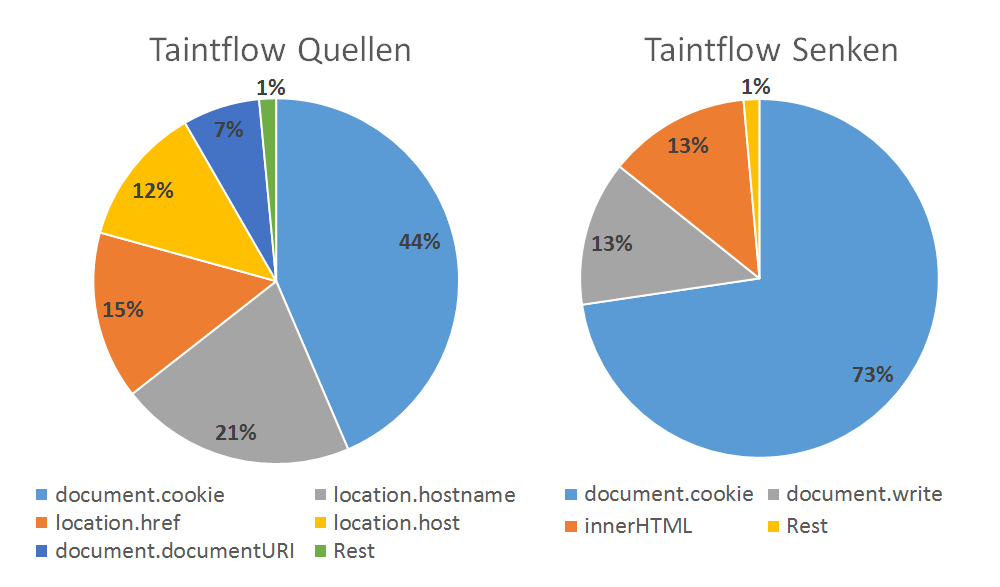
\includegraphics[width=1\textwidth]{Bilder/Diagram1.png}
	\caption{Verteilung der Quellen und Senken von allen Taintflows}
\end{figure}

\section{Webforum}
In Abschnitt XXX wurde ein sehr beschränkter Crawldurchlauf der Alexa Top 500 Webseiten durchgeführt. Dies ist sinnvoll, da so ein fester Datensatz verwendet wurde. In einem zweiten Crawldurchlauf sollen nun viele möglichst verschiedene Seiten besucht werden. Die Hoffnung ist, dadurch so viele Sicherheitslücken wie möglich zu finden.
\subsection{Webcrawler Konfiguration}
Als Startpunkt des Crawlprozesses wird das Webforum reddit.com gewählt, da auf diesem viele externe Links vorhanden sind. Werden auf einer Webseite keine Schwachstellen gefunden, so ist es unwahrscheinlicher auf anderen Webseiten der selben Domäne fündig zu werden. Mit diesem Gedanken im Hinterkopf, wird der Crawler so eingestellt, dass ausschließlich externe Links weiterverfolgt werden. \\
Die maximale Crawltiefe wird auf 7 gestellt, da nur eine einzige Startseite angegeben wurde und es in der Regel nicht so viele externe Links auf einer Seite gibt.
\subsection{Daten zum Crawlvorgang}
Am Ende des Crawlvorgangs wurden insgesamt 1.253.853 Webseiten entdeckt und 75.621 besucht. Das sind etwa gleich viele besuchte Webseiten, wie im vorherigen Versuch. Auf eine Tabelle mit den besuchten Seiten pro Suchtiefe wird hier verzichtet. Die Geschwindigkeit, mit der die Webseiten besucht wurden, ist ebenfalls gleich geblieben. Der Crawlvorgang wurde nach ca. drei Tagen gestoppt.
\subsection{Daten zur Analyse}


\chapter{Fazit}
